\chapter{Trigonometric Ratios}

\section{Introduction}

\subsection{Pythagorean Theorem}

Sea $\Delta ABC$ un triángulo rectángulo, recto en $B$, como se muestra
en la siguiente figura, entonces se cumple que $h^2=a^2+b^2$.

\begin{figure}[ht]
    \centering
    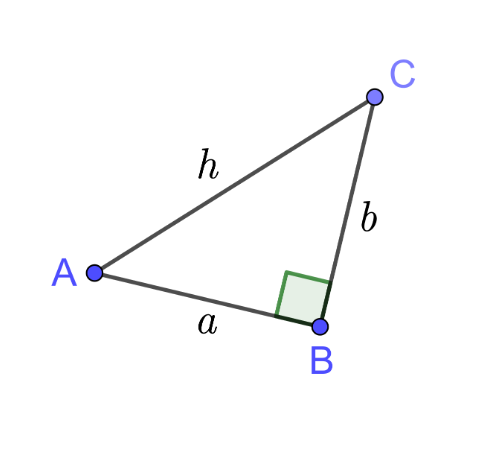
\includegraphics[width=0.3\textwidth]{./images/figure-4.png}
    \caption{Triángulo rectángulo}
    \label{fig:pythagorean_theorem}
\end{figure}

\subsection{Fundamental Identities}

\begin{tabular}{rl}
    $\tan\theta$ &= $\frac{\sin\theta}{\cos\theta}$ \\ 
    \\
    $\cot\theta$ &= $\frac{\cos\theta}{\sin\theta}$ \\
    \\
    $\cot\theta$ &= $\frac{1}{\tan\theta}$ \\
    \\
    $\sec\theta$ &= $\frac{1}{\cos\theta}$ \\
    \\
    $\csc\theta$ &= $\frac{1}{\sin\theta}$ \\
\end{tabular}
